\chapter{システムプログラミング}

本講義は,
オペレーティングシステム本体が持つ機能を直接に使用するような
システムプログラムの作成を行う.
システムプログラムをプログラミングする経験の中から,
オペレーティングシステム本体が備えている機能の役割りや必要性を体感的に学ぶ.

\section{システムプログラムとは}
システムプログラムは,
乱暴な言い方をするとアプリケーション以外のプログラムのことである.
\figref{systemConstruct}にコンピュータシステムの構成を簡単に示す.
この図でアプリケーションプログラムとハードウェアを除いた,
オペレーティングシステム本体(カーネル),
ライブラリ,ミドルウェア,ユーティリティ,プログラム開発環境は
システムプログラムである.

\begin{myfig}{btp}{コンピュータシステムの構成}{systemConstruct}
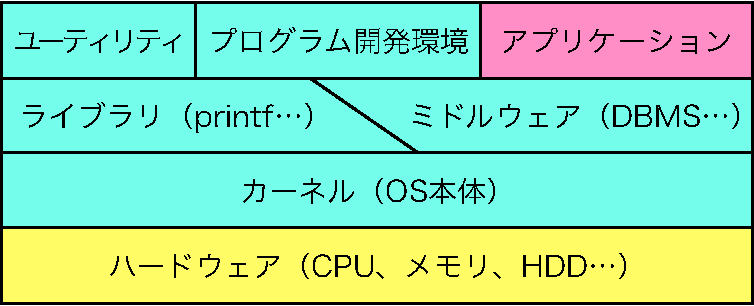
\includegraphics[scale=0.8]{Fig/systemConstruct-crop.pdf}
\end{myfig}

\begin{enumerate}
\item カーネル(OSの本体)
\item ライブラリ(プログラムが使用するサブルーチン,DLL ...)
\item ミドルウェア(DBMS,Webサーバ ...)
\item ユーティリティ(ファイル操作,時計,シェル,システム管理 ...)
\item プログラム開発環境
(エディタ,コンパイラ,アセンブラ,リンカ,インタプリタ ...)
\end{enumerate}

\section{システムプログラミングとは}
システムプログラムを作成することをシステムプログラミングと呼ぶ.
本講義では,
システムプログラムの中でもユーティリティの作成を行う.
WindowsやmacOSではGUIを備えた様々なユーティリティが準備されている\footnote{
WindowsやmacOSの場合でも,
GUIを備えていないユーティリティも,多数,存在する.}.
しかし,本講義の目的は
「システムプログラミングを通してのオペレーティングシステムの体感的な理解」
であるので,GUIの作成にエネルギーを費やしたくはない.
そこで,CLI(Command Line Interface)のユーティリティを作成する.

本講義では,
オペレーティングシステムを体感的に理解するために,
オペレーティングシステムの機能を直接に使用する
\emph{簡単なCLI版のユーティリティプログラムの作成(プログラミング)}を行う.

\section{システムコール}
一つのコンピュータシステムの中で複数のプログラムが同時に作動していることは,
誰もが体験的に知っていると思う.
しかし,それらのプログラムが勝手にシステムの\emph{資源}にアクセスすると,
資源の管理が正しく行えない可能性があり具合が悪い.
例えばハードディスクでは,
複数のプログラムが勝手にファイルを作成すると,
複数のファイルがハードディスクの同じ領域に割当てられるかも知れない.

そこで,
資源にアクセスするのはオペレーティングシステムの
本体である\emph{カーネル}だけに限り,
カーネルが代表して資源を管理することにする.
他のプログラムはカーネルに依頼し目的を達成する.
その様子を図を使って説明する.

\begin{myfig}{btp}{システムコールなし}{noSystemcall}
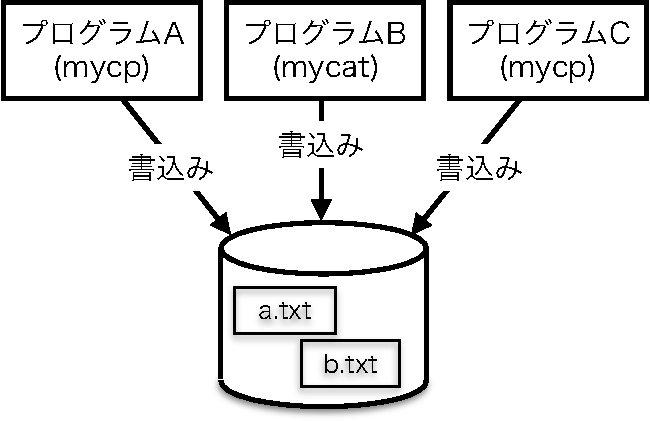
\includegraphics[scale=0.8]{Fig/noSystemcall-crop.pdf}
\end{myfig}

\begin{myfig}{btp}{システムコールあり}{systemcall}
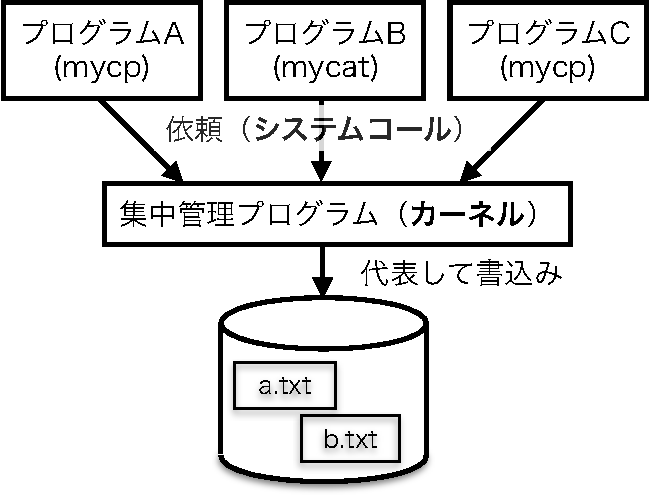
\includegraphics[scale=0.8]{Fig/systemcall-crop.pdf}
\end{myfig}

\begin{enumerate}
\item \figref{noSystemcall}のように,
システムの中で同時に複数のプログラムが実行され,
それぞれが\emph{資源}にアクセスする必要がある.
図の例では,
三つのプログラムが同時にハードディスクにファイルを作ろうとしている.
複数のプログラムが勝手にハードウェア
\emph{資源}(ハードディスク,プリンタ,メモリ ...)を操作すると具合が悪い.
\item そこで,\figref{systemcall}のように資源を集中管理するプログラム,
\emph{カーネル}(OSの本体)を導入する.
一般のプログラムは\emph{システムコール}を用いてカーネルに処理を依頼する.
\end{enumerate}

\section{システムコールの使用}
C言語から,
UNIX(macOS)のシステムコールを直接に利用することが可能である.
以下の章では,
macOS上でC言語を用いてシステムコールを直接に使用するプログラムを作成しながら,
システムコールの機能を確認する.
また,ユーティリティプログラムの簡単版を作成する.

\begin{quote}
\begin{lstlisting}[language=C++, numbers=none]
// ディレクトリを作るユーティリティプログラム(mymkdir)の例
...
int main(int argc, char *argv[]) {
  if (argc!=2) {
    // エラー処理
    ...
  }
  mkdir(argv[1]);    // ディレクトリを作るシステムコール
  return 0;
}
\end{lstlisting}
\end{quote}

\section*{練習問題}
\begin{enumerate}
%\renewcommand{\labelenumi}{\ttfamily \arabic{chapter}.\arabic{enumi}}
% \setlength{\leftskip}{1em}

\item ハードウェア\emph{資源}の例を挙げなさい.

\item \emph{カーネル}の役割りを本章の範囲で説明しなさい.

\item \emph{システムコール}の役割りを簡単に説明しなさい.

\item 自分がいつも使用しているコンピュータやスマートフォンの
オペレーティングシステムの種類(Windows?)を調べなさい.
\end{enumerate}

